\documentclass{ctexart}

\usepackage{cite}
\usepackage{xcolor}
\usepackage{geometry}
\usepackage{fancyhdr}
\usepackage{graphicx}
\usepackage{listings}

\definecolor{codegreen}{rgb}{0,0.6,0}
\definecolor{codegray}{rgb}{0.5,0.5,0.5}
\definecolor{codepurple}{rgb}{0.58,0,0.82}
\definecolor{backcolor}{rgb}{0.95,0.95,0.92}

\lstset{
    backgroundcolor=\color{backcolor},
    commentstyle=\color{codegreen},
    keywordstyle=\color{magenta},
    numberstyle=\tiny\color{codegray},
    stringstyle=\color{codepurple},
    basicstyle=\ttfamily\normalsize,
    breakatwhitespace=false,
    breaklines=true,
    captionpos=b,
    keepspaces=true,
%   numbers=left,
    numbersep=5pt,
    showspaces=false,
    showstringspaces=false,
    showtabs=false,
    tabsize=2
}

\newcommand{\code}[1]{\colorbox{backcolor}{\lstinline|#1|}}

\title{小型搜索引擎的设计与实现}
\author{孙振强}
\date{2021年06月18日}

\begin{document}

    \maketitle
    \newpage

    \tableofcontents
    \newpage


    \section{综述}\label{sec:introduction}

    网页搜索引擎(Web Search Engine)或互联网搜索引擎(Internet Search Engine)是一种用于网络搜索(互联网搜索)的软件系统。搜索引擎在万维网(World Wide Web)上以文本网页搜索的方式获取特定信息。搜索结果通常以一行行的形式显示,其中每行结果为一个网页,该页面被称为搜索引擎结果页面(SERPs, Search Engine Results Pages)。信息包含指向网页、图像、视频、图表、文章、论文及其它类型文件的链接。一些搜索引擎还可以挖掘数据库或开放目录中的数据。不同于仅由人工维护的网页目录,搜索引擎使用网络爬虫来实时维护信息。不能被网页搜索引擎搜索到的互联网内容通常被称为“深网”(Deep Web)\cite{wikipedia-search-engine}。

    目前使用较为广泛的搜索引擎有 Google、Bing、Baidu 等。其中,Google 和 Bing 搜索引擎在全球广泛使用,支持世界上几乎所有语种的语言,提供了对于世界上几乎所有网站的搜索服务。Baidu 搜索引擎在中国广泛使用,对于中文搜索能返回质量较高的搜索结果。除了传统的文本检索模式(Text-Web)外,这三种搜索引擎都提供了多模态检索和跨模态检索的功能,例如语音检索(Voice-Web)、图片检索(Image-Web)、相似图片检索(Image-Image)等功能。

    Google、Bing、Baidu 这些搜索引擎属于全文搜索引擎,此外还有目录搜索引擎、垂直搜索引擎、元搜索引擎\cite{baike-search-engine},下面简要介绍:

    \begin{itemize}
        \item 目录搜索引擎(Index Search Engine):预先设有明确的层级框架,采用人工或半自动的方式检索网页,将网页归档到相应的的目录下。常见的有导航页面和门户网站等;
        \item 全文搜索引擎(Full Text Search Engine):预先爬取网页信息,并建立关键词索引,后根据用户查询的关键词检索数据库,返回相关页面。这是当今主流的搜索引擎,常见的有百度和谷歌等;
        \item 垂直搜索引擎(Vertical Search Engine):针对某个特定领域而建立的专用搜索引擎。相比于全文搜索引擎,垂直搜索引擎的检索范围很小,但能够深入挖掘该领域的专业信息,检索质量较高。常见的有种子搜索引擎、小说搜索引擎、表情包搜索引擎等;
        \item 元搜索引擎(Meta Search Engine):整合多个搜索引擎的结果,并在一个界面上集中展示。元搜索引擎通常没有自己的网络爬虫和数据库,一般实时汇总几个不同搜索引擎的搜索结果。常见的有360综合搜索等;
    \end{itemize}

    此外,一般网站都提供有站内搜索功能,这可以看成一个仅搜索指定站点的小型搜索引擎。例如,在社交媒体网站中通过关键字搜索动态,在电商网站中通过关键词搜索相关商品,在视频网站中通过关键字搜索视频,在新闻网站中通过关键字搜索新闻。

    在这个信息爆炸的时代,互联网上充斥着海量的信息,而搜索引擎能帮我们在短短几秒钟的时间内,搜索到我们想要的结果,这就是搜索引擎的魅力。可以说,网络时代离不开搜索引擎,搜索引擎是人们浏览网络世界的最重要的途径。

    本项目是小型搜索引擎的设计与实现,旨在设计一套完整的搜索引擎系统,实现一个针对特定网站真实可用的搜索引擎系统。本项目紧密围绕课程核心内容,使用 HDFS 和 HBase 进行数据存储,使用 Hadoop MapReduce 进行数据处理,将并行程序设计的思想充分融入到系统的设计之中。本文完全阐述了系统的设计与实现工作,以介绍系统架构开始,再具体介绍四个系统功能模块,后叙述项目进行过程中遇到的困难,最后提出系统在未来的改进之处,并谈谈自己的收获。


    \section{系统架构}\label{sec:archicture}

    本系统采用双节点的服务器集群架构,数据分布式存储在两个节点中,非结构化的数据存储在 HDFS 上,结构化的数据存储在 HBase 上。系统包含四个功能模块,分别是爬虫模块、中文分词模块、PageRank 模块、检索模块。图\ref{fig:archicture} 展示了完整的系统架构。

    本部分从物理架构、数据架构、业务架构三个层次对系统架构进行介绍。图\ref{fig:archicture} 中,绿色的方框表示物理架构部分,橙色的方框表示数据架构部分,蓝色的方框表示业务架构部分。由于 HDFS 和 HBase 架构较为复杂,因此我们使用单独的两节内容分别介绍。

    \begin{figure}[t]
        \centering
        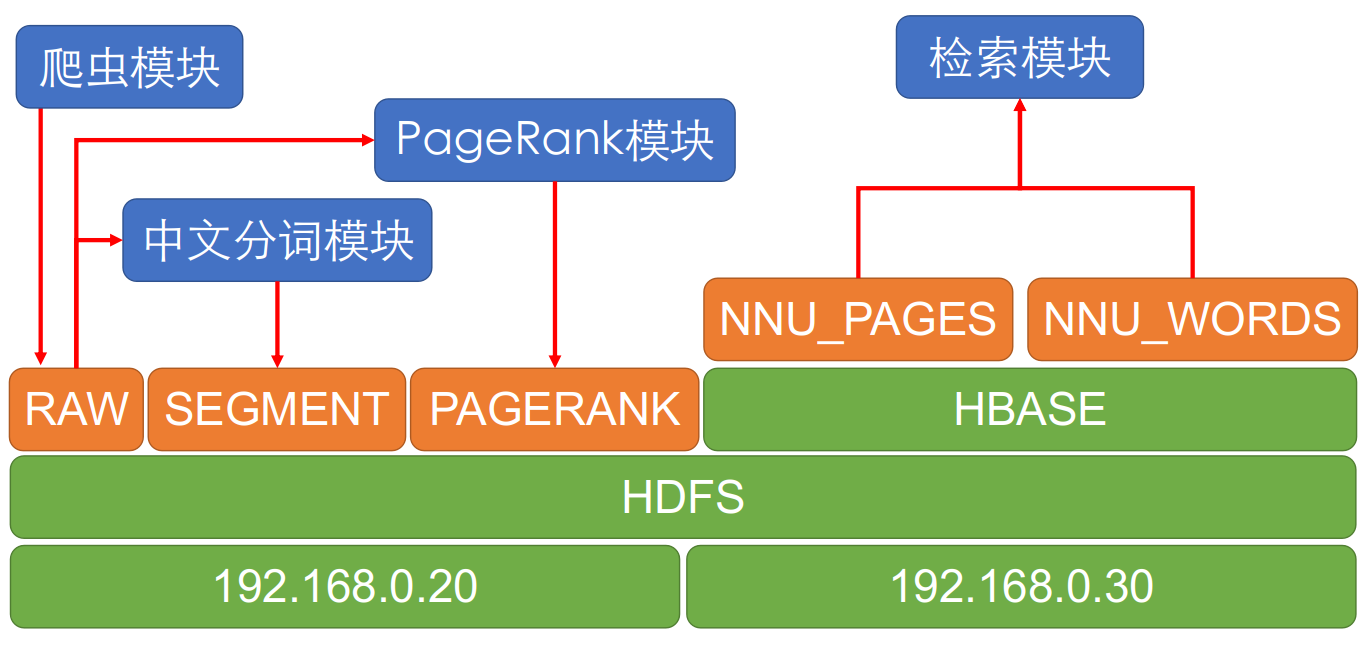
\includegraphics[width=\textwidth]{src/archicture}
        \caption{系统架构示意图}
        \label{fig:archicture}
    \end{figure}

    \subsection{物理架构}\label{subsec:crawl}
    本系统使用了两台学院配发的台式机作为服务器。台式机配置了 Intel(R) Core(TM) i5-6500 CPU @ 3.20GHz 四核四线程的中央处理器,Samsung DIMM DDR4 Synchronous Unbuffered (Unregistered) 2667 MHz 容量为 4 GB 的内存,KINGSTON SV300S3 容量为 120 GB 的固态硬盘,Ubuntu 20.04.2 LTS (Focal Fossa) 的服务器操作系统(无图形化界面)。

    两台服务器位于自己路由器搭建的内网中,表\ref{tab:archicture} 列出了两台服务器的相关配置信息。1 号服务器是主节点,HDFS 的 \code{NameNode} JPS 和 HBase 的 \code{HMaster}、\code{ThriftServer} JPS 均部署在 1 号服务器上。

    注意,jps是一条终端命令,可以列出系统中当前运行的 Java HotSpot VMs\cite{docs-jps},表\ref{tab:archicture} 中的 HDFS JPS 和 HBase JPS 分别代表为 HDFS 和 HBase 提供服务的 Java HotSpot VMs。

    \begin{table}[h]
        \centering
        \caption{服务器配置表}
        \label{tab:archicture}
        \begin{tabular}{c|cccc}
            \hline
            服务器      & 1号服务器         & 2号服务器        \\ \hline
            Hostname & desktop-brown & slaker       \\ \hline
            IP 地址    & 192.168.0.20  & 192.168.0.30 \\ \hline
            HDFS JPS
            & \begin{tabular}{c@{}c@{}}
                  DataNode, NameNode, SecondaryNameNode, \\
                  NodeManager, ResourceManager
            \end{tabular}
            & DataNode \\ \hline
            HBase JPS
            & \begin{tabular}{c@{}c@{}}
                  HRegionServer, HQuorumPeer, \\
                  HMaster, ThriftServer
            \end{tabular}
            & \begin{tabular}{c@{}c@{}}
                  HRegionServer, \\
                  HQuorumPeer
            \end{tabular} \\ \hline
        \end{tabular}
    \end{table}

    \subsection{HDFS 架构}\label{subsec:crawl}

    HDFS 是 Hadoop 分布式文件系统(Hadoop Distributed File System),支持对应用程序数据进行高吞吐量访问\cite{docs-hdfs}。HDFS 是 Hadoop 的一个子模块,因此我们需要在 Hadoop 中配置 HDFS。注意,以下过程建立在单节点配置正确的基础上,请先参照 Hadoop 官方文档\cite{docs-hadoop-single-node} 配置单节点环境。

    打开 \code{core-site.xml} 配置文件,配置 HDFS 在 1 号服务器的 9000 端口上启动,HDFS 存储在每台服务器的 \code{/home/hadoop-\$\{user.name\}} 路径下。修改如下:

    \begin{lstlisting}[language=XML]
<configuration>
    <property>
        <name>fs.defaultFS</name>
        <value>hdfs://desktop-brown:9000</value>
    </property>
    <property>
        <name>hadoop.tmp.dir</name>
        <value>/home/hadoop-${user.name}</value>
    </property>
</configuration>
    \end{lstlisting}

    打开 \code{hdfs-site.xml} 配置文件,将数据副本数量改为一份,即不进行数据冗余备份。修改如下:

    \begin{lstlisting}[language=XML]
<configuration>
    <property>
        <name>dfs.replication</name>
        <value>1</value>
    </property>
</configuration>
    \end{lstlisting}

    打开 \code{workters} 配置文件,添加两台服务器的 hostname:

    \begin{lstlisting}[language=bash]
desktop-brown
slaker
    \end{lstlisting}

    至此,我们将单节点的 HDFS 环境变成了双节点的 HDFS 环境。下面,在 1 号服务器上执行命令格式化 HDFS:

    \begin{lstlisting}[language=bash]
./bin/hdfs namenode -format
    \end{lstlisting}

    接着,执行命令启动 HDFS 和管理器:

    \begin{lstlisting}[language=bash]
./sbin/start-all.sh
    \end{lstlisting}

    我们可以在浏览器中访问 \code{http://192.168.0.20:9870/},查看 HDFS 的运行状态。图\ref{fig:archicture_hdfs-web} 展示了 Namenode 的相关信息,我们可以看到,Namenode 在两台服务器上均已启动并运行。

    \begin{figure}[t]
        \centering
        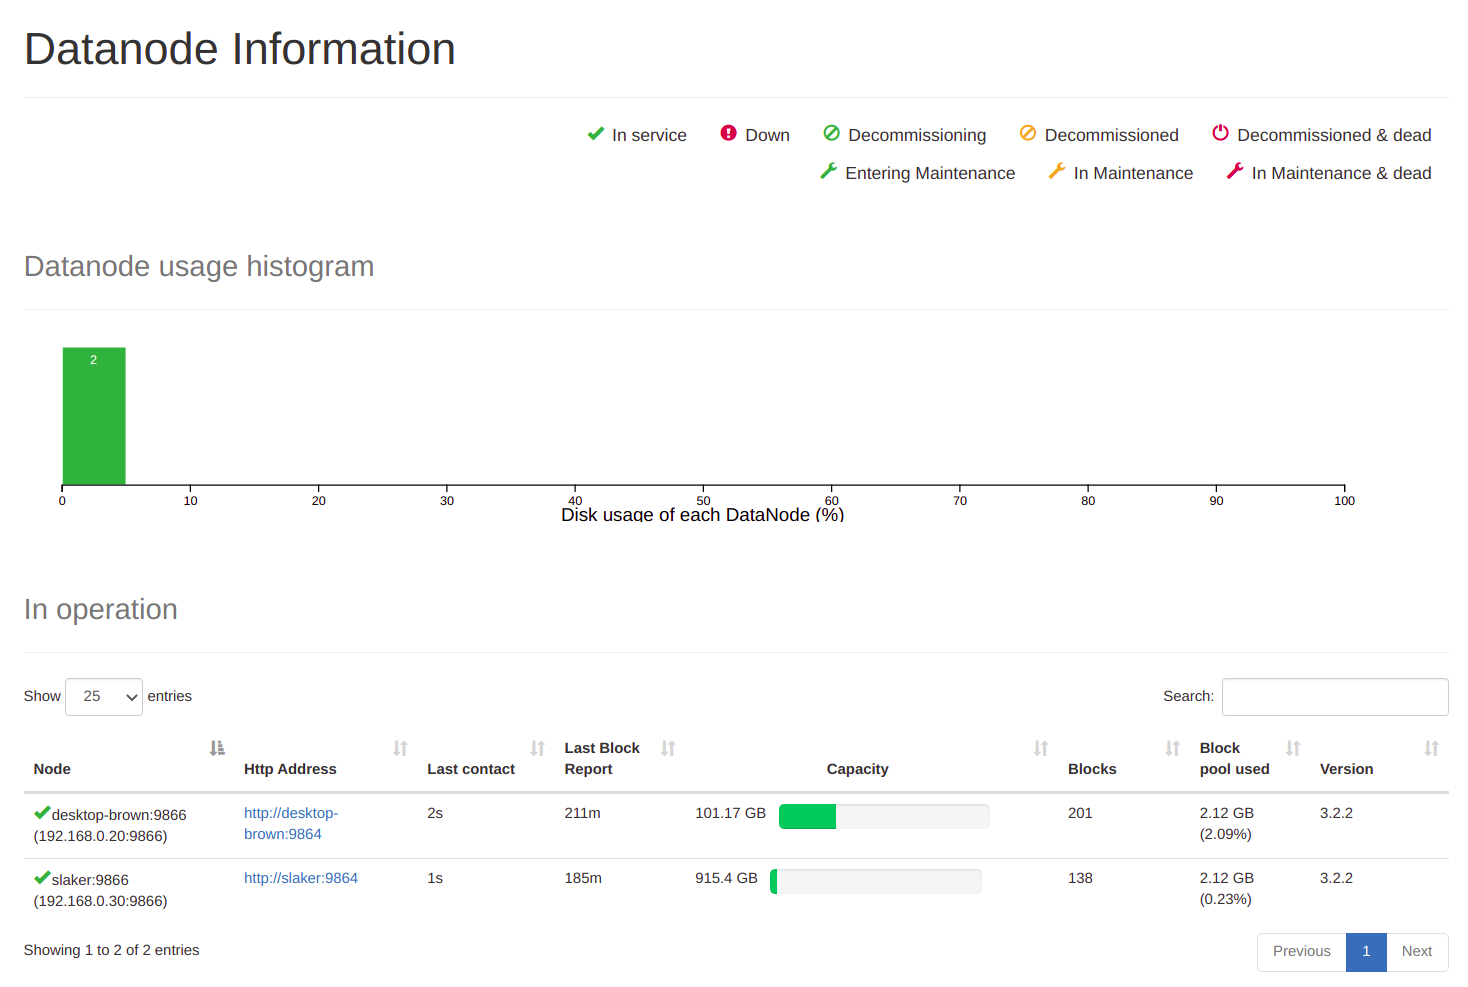
\includegraphics[width=\textwidth]{src/archicture_hdfs-web}
        \caption{HDFS 监控页面}
        \label{fig:archicture_hdfs-web}
    \end{figure}

    \subsection{HBase 架构}\label{subsec:crawl}

    HBase 是 Hadoop 数据库(Hadoop Database),是一个分布式的可拓展的大数据存储数据库\cite{docs-hbase}。下面,我们对 HBase 的配置过程进行简要说明。注意,以下过程省略了在 \code{hbase-env.sh} 文件中对 Java 路径的配置。

    打开 \code{hbase-site.xml} 配置文件,分别配置启动分布式集群部署、路径为 HDFS 根目录下的 code 文件夹、zookeeper 要管理的两台服务器的 hostname、zookeeper 数据存储路径。修改如下:

    \begin{lstlisting}[language=XML]
<configuration>
  <property>
    <name>hbase.cluster.distributed</name>
    <value>true</value>
  </property>
  <property>
    <name>hbase.rootdir</name>
    <value>hdfs://desktop-brown:9000/hbase</value>
  </property>
  <property>
    <name>hbase.zookeeper.quorum</name>
    <value>desktop-brown,slaker</value>
  </property>
  <property>
    <name>hbase.zookeeper.property.dataDir</name>
    <value>/home/zookeeper</value>
  </property>
</configuration>
    \end{lstlisting}

    打开 \code{regionservers} 配置文件,添加两台服务器的 hostname:

    \begin{lstlisting}[language=bash]
desktop-brown
slaker
    \end{lstlisting}

    至此,我们完成了双节点 HBase 的配置工作。下面,在 1 号服务器上执行命令启动 HBase:

    \begin{lstlisting}[language=bash]
./bin/start-hbase.sh
    \end{lstlisting}

    接着,执行命令启动 Thrift 服务器:

    \begin{lstlisting}[language=bash]
./bin/hbase thrift start
    \end{lstlisting}

    我们可以在浏览器中访问 \code{http://192.168.0.20:16010/},查看 HBase 的运行状态。图\ref{fig:archicture_hbase-web} 展示了 HBase 的相关信息,我们可以看到,Region Servers 在两台服务器上均已启动并运行。

    \begin{figure}[t]
        \centering
        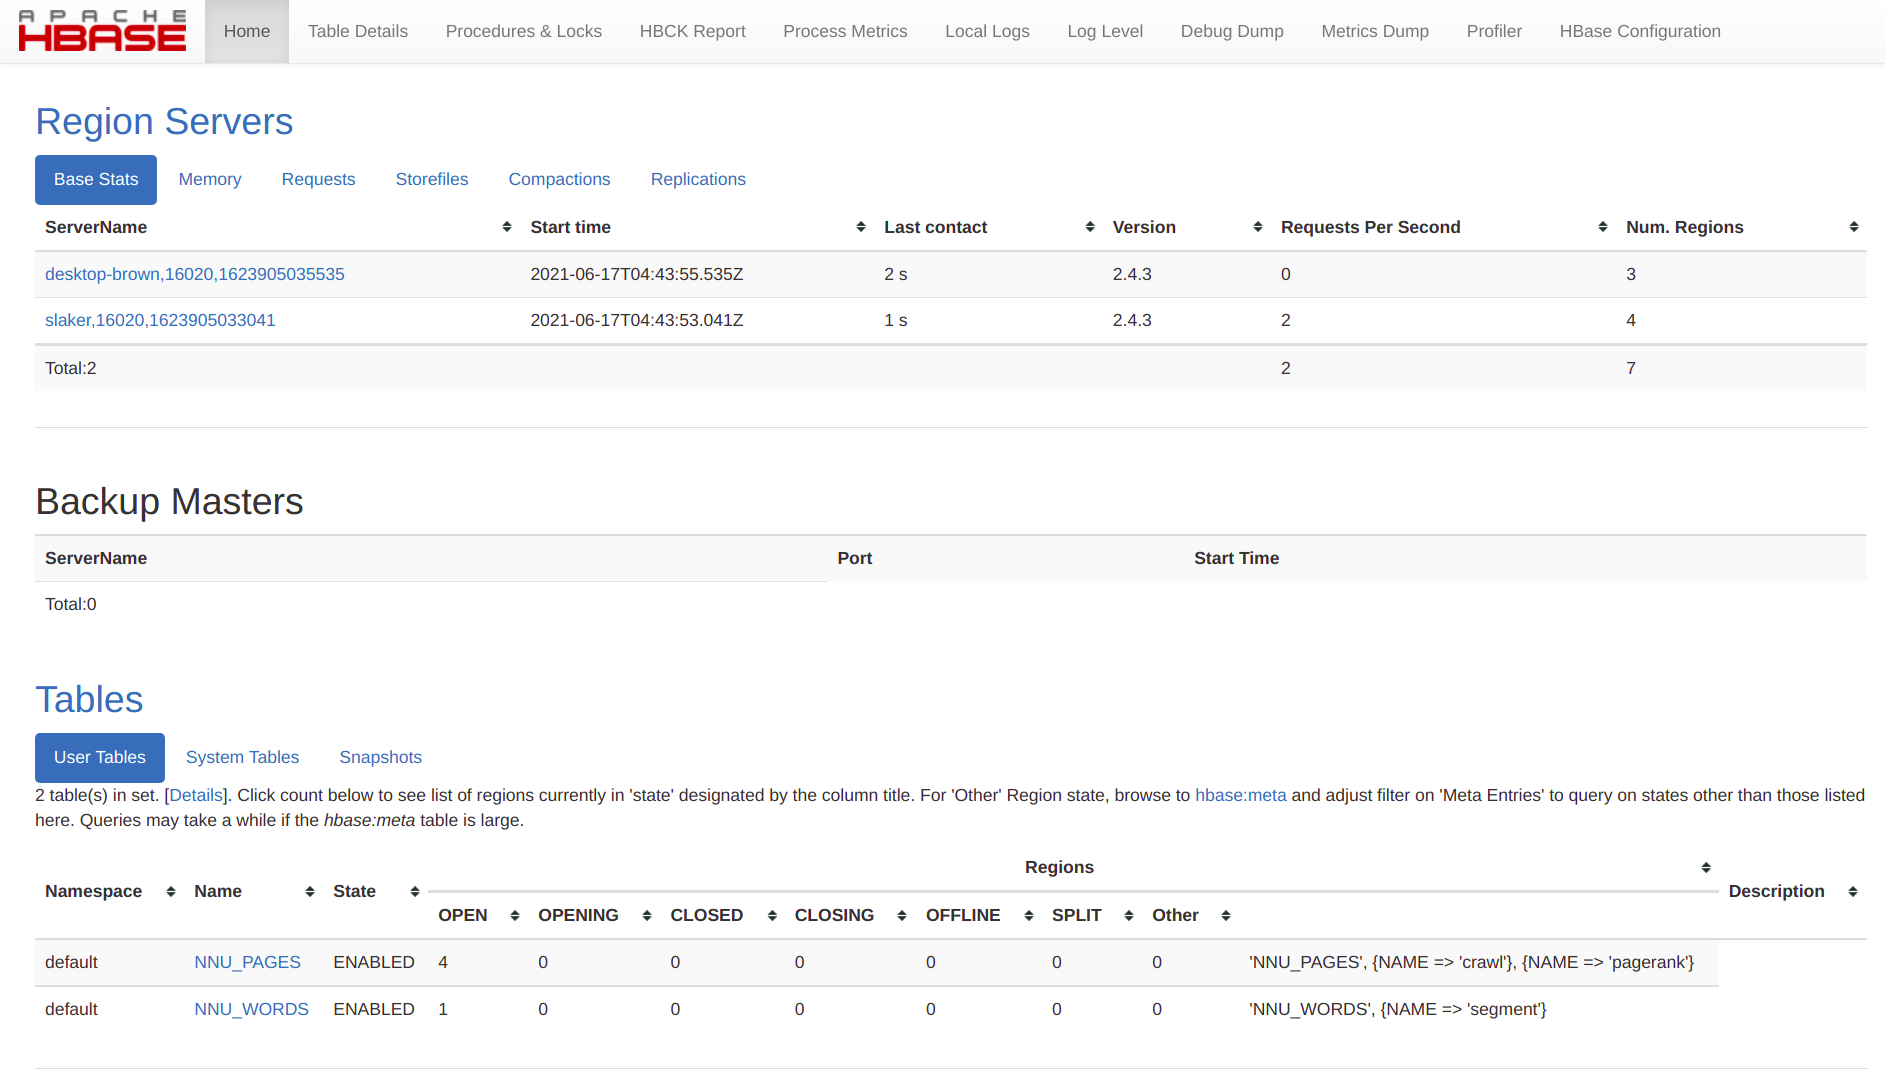
\includegraphics[width=\textwidth]{src/archicture_hbase-web}
        \caption{HBase 监控页面}
        \label{fig:archicture_hbase-web}
    \end{figure}

    \subsection{数据架构}\label{subsec:crawl}

    系统的所有数据均存储在 HDFS 和 HBase 上。其中,非结构化数据 \code{RAW}、\code{SEGMENT}、\code{PAGERANK} 存储在 HDFS 上,结构化数据 \code{NNU_PAGES}、\code{NNU_WORDS} 存储在 HBase 上。下面对这五部分的数据进行简要说明:

    \begin{itemize}
        \item \code{RAW}:爬虫模块爬取得到的网页原始数据,记录了每个页面的 URL、页面内包含的超链接、标题和正文内容;
        \item \code{SEGMENT}:经过中文分词模块处理后得到的数据,记录了每个关键词及包含该关键词的所有 URL;
        \item \code{PAGERANK}:经过 PageRank 模块处理后得到的数据,记录了每个页面的 URL 及其 PageRank 值;
        \item \code{NNU_PAGES}:HBase 中的一张表,记录了每个页面的所有信息,表结构及样例数据如表\ref{tab:archicture_nnu-pages} 所示。该表包含两个 column family \code{crawl} 和 \code{pagerank},分别代表由爬虫模块和 PageRank 模块产生的数据;
        \item \code{NNU_WORDS}:HBase 中的一张表,记录了每个关键词的所有信息,表结构及样例数据如表\ref{tab:archicture_nnu-words} 所示。该表包含一个 column family \code{segment},代表由中文分词模块产生的数据。我们会在第 \ref{subsec:segment} 节中说明 \code{segment:URLs} 字段的数据格式;
    \end{itemize}

    \begin{table}[h]
        \centering
        \caption{NNU\_PAGES 表及样例数据}
        \label{tab:archicture_nnu-pages}
        \begin{tabular}{c|cccc}
            \hline
            ID        & crawl:title & crawl:body & crawl:nextURLs      & pagerank:value \\ \hline
            www.1.com & title-1     & body-1     & www.2.com www.3.com & 1.64           \\
            www.2.com & title-2     & body-2     & www.1.com           & 0.88           \\
            www.3.com & title-3     & body-3     &                     & 0.32           \\ \hline
        \end{tabular}
    \end{table}

    \begin{table}[h]
        \centering
        \caption{NNU\_WORDS 表及样例数据}
        \label{tab:archicture_nnu-words}
        \begin{tabular}{c|cccc}
            \hline
            ID     & segment:URLs                                 \\ \hline
            hello  & www.1.com@@1-5 www.2.com@23-27 www.3.com@0-4 \\
            hadoop & www.2.com@@2-7                               \\
            hbase  & www.1.com@@2-6 www.3.com@101-105             \\ \hline
        \end{tabular}
    \end{table}

    \subsection{业务架构}\label{subsec:crawl}

    系统包含四个功能模块,分别处理一个完整的业务逻辑。下面对这四个功能模块进行简要说明:

    \begin{itemize}
        \item 爬虫模块:从互联网上爬取指定站点的网页内容,解析每个页面的 URL、页面内包含的超链接、标题和正文内容,输出 \code{RAW} 数据,并迁移至 \code{NNU_PAGES} 表的 \code{crawl} 族中;
        \item 中文分词模块:输入 \code{RAW} 数据,使用 Hadoop MapReduce 对每个页面的标题和正文内容进行分词,对于每个关键词,收集所有含有该关键词的 URL 及关键词在页面中出现的位置,输出 \code{SEGMENT} 数据,并迁移至 \code{NNU_PAGES} 表的 \code{segment} 族中;
        \item PageRank 模块:输入 \code{RAW} 数据,使用 Hadoop MapReduce 迭代地计算每个页面的 PageRank 值,输出 \code{PAGERANK} 数据,并迁移至 \code{NNU_PAGES} 表的 \code{pagerank} 族中;
        \item 检索模块:输入 \code{NNU_PAGES} 和 \code{NNU_WORDS} 数据和查询关键词,先从 \code{NNU_WORDS} 表中筛选出包含该关键词的所有页面,再从 \code{NNU_WORDS} 表中读取这些页面的信息,排序并高亮关键词后输出搜索结果;
    \end{itemize}


    \section{功能模块设计}\label{sec:modules}

    本章我们将详细阐述系统爬虫模块、中文分词模块、PageRank 模块、检索模块这四个功能模块的设计,包括每个模块的输入数据说明、数据处理过程、输出数据说明。

    \subsection{爬虫模块}\label{subsec:crawl}

    爬虫模块的目的是从互联网上爬取并解析网页数据,使用 Java 多线程进行并行爬虫作业。开始时,给定入口网页地址和域名限制范围,每次爬取并解析完一个页面后,将页面内容保存到磁盘中,将该页面添加到“完成集合”中,以后再遇到该页面将不再重复爬取,将该页面中包含的所有超链接加入到“等待队列”中,直到“等待队列”为空才结束。

    \subsubsection{爬虫范围}\label{subsubsec:crawl_scope}

    本项目的爬虫范围是“南京师范大学”的部分网页,包括南京师范大学的主站点、阳光网、研究生院(研工部)、所有 28 个二级学院的网站。完整的域名范围如表\ref{tab:crawl_domains} 所示。其中,阳光网是南京师范大学发布各类新闻咨询的网站。

    \begin{table}[h]
        \centering
        \caption{爬虫的域名限制范围}
        \label{tab:crawl_domains}
        \scriptsize{
            \begin{tabular}{ccl|ccl}
                \hline
                序号 & 域名                 & 说明              & 序号 & 域名                   & 说明                  \\ \hline
                1  & www.njnu.edu.cn    & 南京师范大学主站点       & 17 & xinchuan.njnu.edu.cn & 新闻与传播学院             \\
                2  & news.njnu.edu.cn   & 南京师范大学阳光网       & 18 & sfy.njnu.edu.cn      & 社会发展学院              \\
                3  & grad.njnu.edu.cn   & 南京师范大学研究生院(研工部) & 19 & math.njnu.edu.cn     & 数学科学学院              \\
                4  & honors.njnu.edu.cn & 强化培养学院          & 20 & physics.njnu.edu.cn  & 物理科学与技术学院           \\
                5  & jsjyxy.njnu.edu.cn & 教师教育学院          & 21 & hky.njnu.edu.cn      & 化学与材料科学学院           \\
                6  & gjy.njnu.edu.cn    & 国际文化教育学院        & 22 & dky.njnu.edu.cn      & 地理科学学院              \\
                7  & jny.njnu.edu.cn    & 金陵女子学院          & 23 & sky.njnu.edu.cn      & 生命科学学院              \\
                8  & spa.njnu.edu.cn    & 公共管理学院          & 24 & energy.njnu.edu.cn   & 能源与机械工程学院           \\
                9  & sxy.njnu.edu.cn    & 商学院             & 25 & d.njnu.edu.cn        & 电气与自动化工程学院          \\
                10 & law.njnu.edu.cn    & 法学院             & 26 & ceai.njnu.edu.cn     & 计算机与电子信息学院 / 人工智能学院 \\
                11 & marx.njnu.edu.cn   & 马克思主义学院         & 27 & env.njnu.edu.cn      & 环境学院                \\
                12 & jky.njnu.edu.cn    & 教育科学学院          & 28 & hy.njnu.edu.cn       & 海洋科学与工程学院           \\
                13 & xlxy.njnu.edu.cn   & 心理学院            & 29 & spxy.njnu.edu.cn     & 食品与制药工程学院           \\
                14 & tky.njnu.edu.cn    & 体育科学学院          & 30 & music.njnu.edu.cn    & 音乐学院                \\
                15 & wxy.njnu.edu.cn    & 文学院             & 31 & msxy.njnu.edu.cn     & 美术学院                \\
                16 & wy.njnu.edu.cn     & 外国语学院           &    &                      &                     \\ \hline
            \end{tabular}
        }
    \end{table}

    \subsubsection{爬虫过程}\label{subsubsec:crawl_run}

    爬虫模块的整体架构如图\ref{fig:crawl} 所示。其中,蓝色 Thread 方框是由 Java 线程池维护的一系列线程,绿色 \code{WAIT\_URL\_POOL} 和 \code{FINISH\_URL\_POOL} 方框分别是“等待队列”和“完成集合”,橙色 \code{RAW} 方框是存储的网页数据。

    爬虫过程的算法叙述如下:

    \begin{enumerate}
        \item 设置参数:指定入口页面为南京师范大学首页(http://www.njnu.edu.cn/)并设置域名范围,指定 Java 线程池的线程个数;
        \item 初始化:将入口网页添加到 \code{WAIT\_URL\_POOL} 中,初始化 Java 线程池;
        \item 请求:线程池中的每个线程,若当前为空闲状态,则从 \code{WAIT\_URL\_POOL} 中取出一个 URL,请求 html 文档;
        \item 解析:从 html 文档中解析出标题(title)、正文(body)、包含的超链接(nextURLs);
        \item 保存:将 URL、title、body、nextURLs 保存到磁盘中;
        \item 添加 nextURLs:对于 nextURLs 中的每个 nextURL,若不在 \code{FINISH\_URL\_POOL} 中且在域名范围内,则将 nextURL 添加到 \code{WAIT\_URL\_POOL} 中;
        \item 移 URL:从 \code{WAIT\_URL\_POOL} 中移除当前 URL;
        \item 若 \code{WAIT\_URL\_POOL} 不为空,返回第 3 步;
        \item 程序结束;
    \end{enumerate}

    下面对爬虫程序做几点说明:

    \begin{itemize}
        \item 程序中使用 \code{Jsoup} 包操作 html 文档,可以非常方便地进行请求网页、提取超链接、过滤 html 格式等操作;
        \item 在 \code{WAIT\_URL\_POOL} 和 \code{FINISH\_URL\_POOL} 中,使用了 \code{java.util.UUID} 以加快判重效率;
        \item 会出现形如 “www.1.com/hello#tab” 的 URL,后面的 “#tab” 是网页内部的锚点定位,需要过滤掉,变成 “www.1.com/hello”,不然爬虫程序会重复爬取相同页面,大大增加数据量;
        \item 在第 5 步保存时,保存函数 save() 使用了 \code{synchronized} 关键字,执行串行化存储过程,以防止多线程出现数据丢失或不同步的问题;
    \end{itemize}

    \begin{figure}[t]
        \centering
        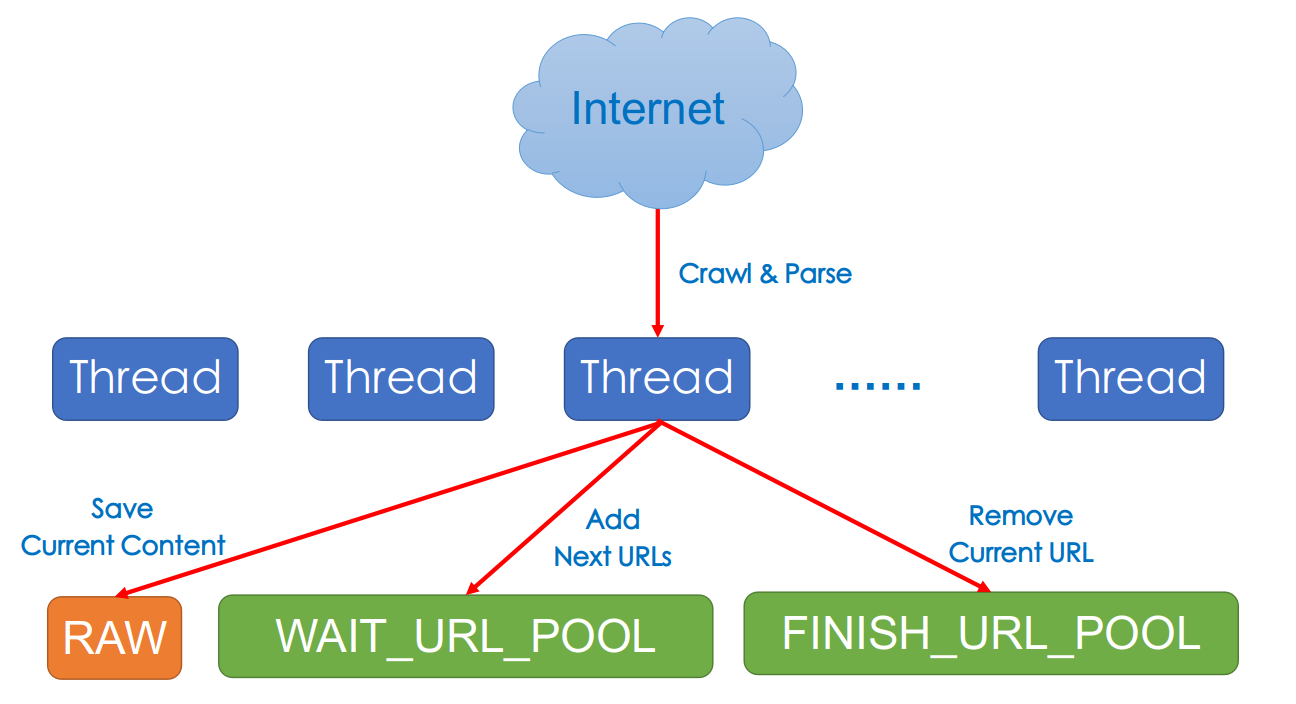
\includegraphics[width=\textwidth]{src/crawl}
        \caption{爬虫模块架构示意图}
        \label{fig:crawl}
    \end{figure}

    \subsubsection{RAW 数据}\label{subsubsec:crawl_data}

    爬虫得到的数据分块存储在磁盘中,如图\ref{fig:crawl_files} 所示。具体来说,每个页面需要保存四个字段:URL、nextURLs、title、body,每个页面占用一行。每个文件中存储 10000 个页面,即每个文件有 10000 行。若文件超过 10000 行,则会创建一个新文件来保存数据,文件名按照格式 \code{part-0}、\code{part-1}、\code{part-2} …… 顺序编号。下面展示了一个 \code{part-*} 文件的结构样例。注意,每个 \code{[xxx]} 是一个字段名,字段名和内容之间使用分隔符 “\verb|\|t” 隔开,因此 title 和 body 中的 “\verb|\|t” 字符需要全部过滤掉。

    \begin{lstlisting}[basicstyle=\ttfamily\footnotesize]
[0]    [URL] www.1.com    [nextURLs] www.2.com www.3.com [title] title-1    [body] body-1
[1]    [URL] www.2.com    [nextURLs] www.1.com           [title] title-2    [body] body-2
[2]    [URL] www.3.com    [nextURLs]                     [title] title-3    [body] body-3
…… …… …… …… …… …… …… …… …… …… …… …… …… …… …… …… …… ……
[9999] [URL] www.9999.com [nextURLs] www.1.com www.8.com [title] title-9999 [body] body-9999
    \end{lstlisting}

    \begin{figure}[h]
        \centering
        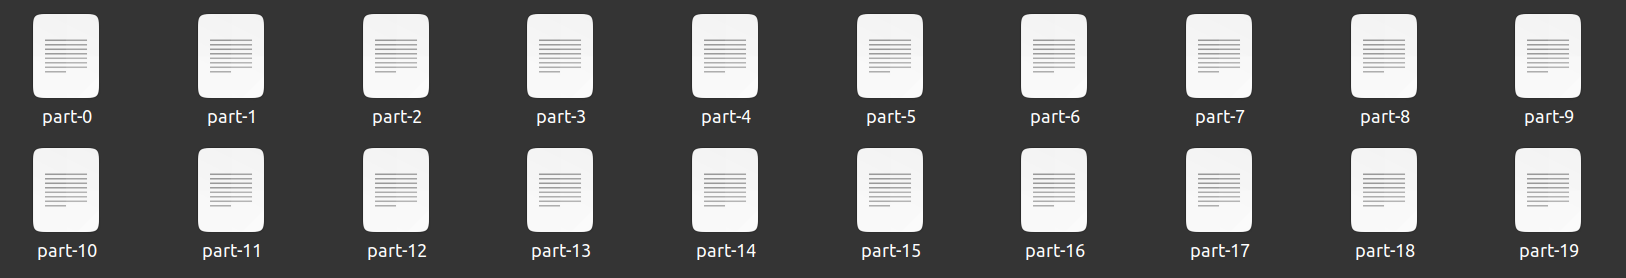
\includegraphics[width=\textwidth]{src/crawl_files}
        \caption{分块存储的网页数据}
        \label{fig:crawl_files}
    \end{figure}

    图\ref{fig:crawl_row} 是南京师范大学首页在文件中的真实数据。可以看到,\code{[URL]} 字段是 http://www.njnu.edu.cn/,\code{[nextURLs]} 字段中有非常多的超链接,\code{[title]} 字段是 “南京师范大学”,\code{[body]} 字段是网页中的纯文本内容。

    \begin{figure}[t]
        \centering
        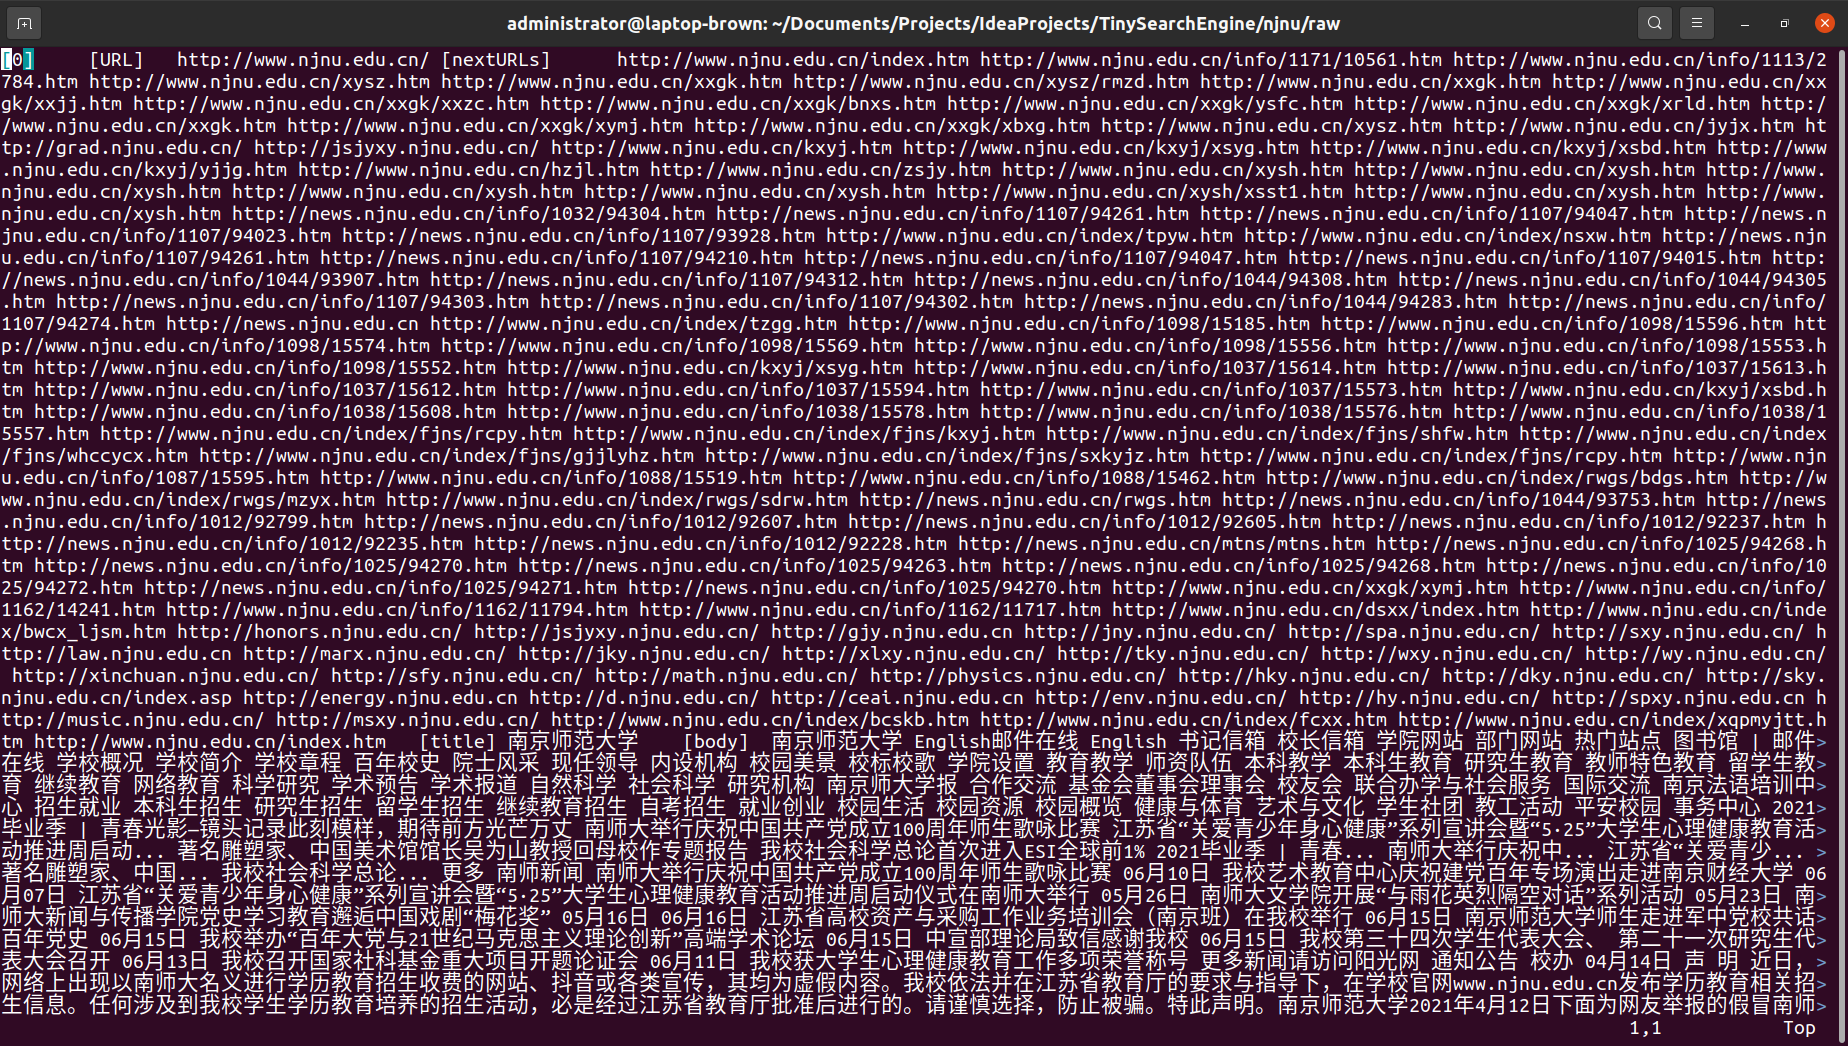
\includegraphics[width=\textwidth]{src/crawl_row}
        \caption{南京师范大学首页在分块文件中存储的数据}
        \label{fig:crawl_row}
    \end{figure}

    \subsubsection{迁移到 HBase}\label{subsubsec:crawl_migrate}

    最后,我们将分块文件中的数据迁移到 HBase 的 \code{NNU\_PAGES} 表的 \code{crawl} 族中,\code{NNU\_PAGES} 表的结构如表\ref{tab:archicture_nnu-pages} 所示。文件 \code{[URL]} 字段是每条记录的 \code{ID},文件 \code{[nextURLs]} 字段对应表中的 \code{crawl:nextURLs} 字段,文件 \code{[title]} 字段对应表中的 \code{crawl:title} 字段,文件 \code{[body]} 字段对应表中的 \code{crawl:body} 字段。

    \subsection{中文分词模块}\label{subsec:segment}

    \subsection{PageRank模块}\label{subsec:pagerank}

    \subsection{检索模块}\label{subsec:retrieve}


    \section{项目演示}\label{sec:demo}
    1


    \section{遇到的困难}\label{sec:difficulty}

    2\cite{pascal} 123312\cite{search-engine}


    \section{未来的改进}\label{sec:improvement}


    \section{自己的收获}\label{sec:achievement}

    \bibliographystyle{unsrt}
    \bibliography{references}

\end{document}